% ============================================================
%  Embedding-Space vs. Accuracy-Based Drift Detection
%  for Open-Source LLMs: A Controlled Comparative Study
%
%  AITR Lab 02 — MRA14 — AI Tools for Research (Post Mid-Sem)
%  Single-column format
%  Compile: pdflatex main.tex  (twice)
%           bibtex  main
%           pdflatex main.tex
%           pdflatex main.tex
% ============================================================

\documentclass[12pt,a4paper]{article}

% ── Margins ──────────────────────────────────────────────────────────────────
\usepackage[top=2.5cm, bottom=2.5cm, left=2.5cm, right=2.5cm]{geometry}

% ── Packages ─────────────────────────────────────────────────────────────────
\usepackage{cite}
\usepackage{amsmath,amssymb,amsfonts}
\usepackage{graphicx}
\usepackage{textcomp}
\usepackage{xcolor}
\usepackage{booktabs}
\usepackage{multirow}
\usepackage{url}
\usepackage{hyperref}
\usepackage{float}
\usepackage{algorithm}
\usepackage{algorithmic}
\usepackage{setspace}
\usepackage{titlesec}
\usepackage{abstract}
\usepackage{parskip}

\onehalfspacing

\hypersetup{
  colorlinks = true,
  linkcolor  = blue!70!black,
  citecolor  = blue!70!black,
  urlcolor   = blue!70!black,
}

% ── Section style ─────────────────────────────────────────────────────────────
\titleformat{\section}{\large\bfseries}{\thesection.}{0.5em}{}
\titleformat{\subsection}{\normalsize\bfseries}{\thesubsection.}{0.5em}{}
\titleformat{\subsubsection}{\normalsize\itshape}{\thesubsubsection.}{0.5em}{}

% ── Title ────────────────────────────────────────────────────────────────────
\title{\Large\textbf{Embedding-Space vs.\ Accuracy-Based Drift Detection\\
for Open-Source LLMs: A Controlled Comparative Study}}

\author{
  \textbf{MRA2026014 - VAASU MAROTHIA}\\[4pt]
  \textit{AI Tools for Research — Post Mid-Semester Assignment}\\
  \textit{[IIIT Allahabad]}
}

\date{}

% =============================================================================
\begin{document}

\maketitle
\thispagestyle{empty}

% ── Abstract ─────────────────────────────────────────────────────────────────
\begin{abstract}
Recent reports document measurable temporal performance drift in large language
models (LLMs) deployed via public APIs~\cite{Chen2023,Ouyang2022}. Continuously
re-evaluating task accuracy is both expensive and label-dependent.  We
investigate whether embedding-space distributional metrics—Jensen-Shannon
Divergence~\cite{Lin1991} (JSD) over output logit distributions and Maximum
Mean Discrepancy~\cite{Gretton2012} (MMD) over Sentence-BERT
embeddings~\cite{Reimers2019}—can serve as reliable, label-free early-warning
indicators of drift in open-source LLMs.  We conduct a controlled comparative
study on GPT-2-medium and DistilGPT-2~\cite{Radford2019,Sanh2019} evaluated on
a temporally partitioned subset of TriviaQA~\cite{Joshi2017}, simulating
knowledge-domain distribution shift.  Three monitoring approaches are compared:
accuracy-based monitoring (\textsc{ACC-MON}), output-distribution JSD monitoring
(\textsc{JSD-MON}), and sentence-embedding MMD monitoring (\textsc{MMD-MON}).
Under controlled domain shift, \textsc{JSD-MON} achieves the highest
AUC-ROC of 0.93 on DistilGPT-2 and detects drift as early as 1~sample
after onset on GPT-2-medium, while \textsc{MMD-MON} achieves the lowest false
positive rate (FPR\,=\,0.28 at TPR\,=\,0.90).  Both label-free monitors
consistently outperform \textsc{ACC-MON} in AUC-ROC.  A window-size ablation
identifies $w\!=\!125$~samples as optimal for \textsc{MMD-MON} (AUC\,=\,0.98,
FPR\,=\,0.08).  Our code and results are publicly available.

\medskip\noindent\textbf{Keywords:} large language models, performance drift,
distribution shift, drift detection, sentence embeddings, TriviaQA, GPT-2
\end{abstract}

\newpage
\newpage

% =============================================================================
\section{Introduction}
\label{sec:intro}

Large language models are increasingly integrated into production systems, from
customer-facing chatbots to scientific literature assistants.  Unlike classical
ML pipelines, LLMs offered through cloud APIs are frequently updated silently,
exposing downstream applications to unexpected behavioral changes without
explicit version notifications.

Chen~et~al.~\cite{Chen2023} empirically demonstrated that GPT-3.5-turbo and
GPT-4 exhibit statistically significant drift in code generation, math reasoning,
and content-sensitivity tasks over a five-month observation window (March–July
2023).  Among other findings, they report a drop of more than 50~percentage points
in the fraction of sensitive questions answered by GPT-4.  Ouyang~et~al.~\cite{Ouyang2022}
document how instruction fine-tuning substantially reshapes model behavior,
illustrating that model updates fundamentally alter output distributions.  These
findings underscore the operational risk of assuming LLM stability.

The standard response to drift—periodic accuracy re-evaluation on labelled test
sets—is expensive, requires maintained annotation pipelines, and can only alert
operators \emph{after} drift has already accumulated into measurable performance
loss.  An alternative paradigm, adapted from classical concept drift
detection~\cite{Gama2014,Lu2018}, monitors the statistical properties of model
outputs in an unsupervised or weakly supervised manner, ideally flagging drift
before it manifests in task metrics.

This paper addresses the following primary research question:
\begin{quote}
\textit{Do embedding-space distributional metrics (JSD, MMD) provide earlier
and more reliable detection of task-performance degradation than accuracy-based
monitoring in open-source LLMs under controlled domain distribution shift?}
\end{quote}

We further ask: (Q2)~\textit{Does increasing the sliding window size improve
detection reliability at the cost of detection delay?}

\noindent Our contributions are:
\begin{enumerate}
  \item A reproducible controlled drift experiment using open-source models and a
        freely available dataset, with protocol frozen before result inspection.
  \item An empirical comparison of three monitoring approaches—\textsc{ACC-MON},
        \textsc{JSD-MON}, \textsc{MMD-MON}—on two model scales.
  \item An ablation study on sliding window size, characterising the
        sensitivity–delay trade-off.
  \item All code, results, and configurations released in the companion repository.
\end{enumerate}

% =============================================================================
\section{Related Work}
\label{sec:related}

\subsection{LLM Temporal Drift}
Chen~et~al.~\cite{Chen2023} provide the first systematic empirical study of
temporal behavioral drift in proprietary LLMs.  Their methodology of repeated
standardised evaluation at fixed intervals inspired our controlled simulation
approach.  Ouyang~et~al.~\cite{Ouyang2022} show that instruction fine-tuning
(InstructGPT) reshapes output distributions; silently updated models therefore
constitute a real operational risk.  Liang~et~al.~\cite{Liang2022} propose
HELM, a holistic LLM evaluation suite measuring performance across multiple
axes; we adopt their emphasis on consistent evaluation protocols and transparent
reporting.

\subsection{Concept Drift Detection}
Classical concept drift detection~\cite{Gama2014} distinguishes virtual drift
($P(X)$ shifts, $P(Y\mid X)$ unchanged) from real drift ($P(Y\mid X)$ shifts).
Statistical tests—Kolmogorov-Smirnov, Population Stability Index, sliding-window
mean comparison—have been widely applied to tabular and image streams.
Lu~et~al.~\cite{Lu2018} survey deep-learning-based approaches.  LLM drift most
closely resembles real drift, but can manifest as virtual drift when the user's
prompt distribution shifts.

\subsection{Distributional Similarity Metrics}
Jensen-Shannon Divergence~\cite{Lin1991} is a symmetric, bounded variant of
KL divergence, natural for comparing discrete probability distributions such as
token-level logit outputs.  Maximum Mean Discrepancy~\cite{Gretton2012} is a
kernel-based metric comparing two distributions in reproducing kernel Hilbert
space; it applies to continuous embedding vectors and is consistent under
mild conditions.  Reimers and Gurevych~\cite{Reimers2019} demonstrate that
sentence-level BERT embeddings encode rich semantic information, making them
suitable inputs for distributional comparison.  Prior work has applied MMD to
detect dataset shift in computer vision; our study extends this to LLM output
monitoring.

% =============================================================================
\section{Methodology}
\label{sec:method}

We define the drift detection problem as follows.  A reference window
$\mathcal{R}=\{z_1,\ldots,z_m\}$ of model outputs is collected under
in-distribution conditions.  A test stream
$\mathcal{S}=\{s_1,s_2,\ldots\}$ is processed sequentially; drift is declared
when a test statistic computed over the most recent $w$~samples in~$\mathcal{S}$
exceeds a threshold calibrated on~$\mathcal{R}$.

\subsection{Accuracy-Based Monitoring (\textsc{ACC-MON})}
\textsc{ACC-MON} maintains a sliding window of size~$w$ over binary correctness
labels.  Drift is flagged when the rolling accuracy drops by more than
$\delta_\mathrm{acc}$ below the reference accuracy~$\bar{a}_\mathcal{R}$:
\begin{equation}
\hat{a}_t = \frac{1}{w}\sum_{i=t-w+1}^{t} y_i,\quad
\text{flag if}\quad \bar{a}_\mathcal{R} - \hat{a}_t > \delta_\mathrm{acc}.
\label{eq:acc}
\end{equation}
\textsc{ACC-MON} requires ground-truth labels at test time and is provided as
the primary baseline reflecting current operational practice.

\subsection{JSD-Based Monitoring (\textsc{JSD-MON})}
At each step, the LLM produces a logit vector over its vocabulary.  We compute
a soft probability distribution $p_t=\mathrm{softmax}(\ell_t)$ and average over
the sliding window.  \textsc{JSD-MON} flags drift when:
\begin{equation}
\mathrm{JSD}(\bar{p}_\mathcal{R}\,\|\,\bar{p}_t)>\delta_\mathrm{jsd},
\label{eq:jsd}
\end{equation}
where $\bar{p}_\mathcal{R}$ is the reference average,
$\bar{p}_t=\frac{1}{w}\sum_{i=t-w+1}^{t}p_i$, and
\begin{equation}
\mathrm{JSD}(P\|Q)=\tfrac{1}{2}D_\mathrm{KL}(P\|M)+\tfrac{1}{2}D_\mathrm{KL}(Q\|M),\quad
M=\tfrac{P+Q}{2}.
\end{equation}
JSD is bounded in $[0,\ln 2]$, permitting consistent threshold calibration across
models and vocabulary sizes.

\subsection{MMD-Based Monitoring (\textsc{MMD-MON})}
Each input question is encoded by a frozen Sentence-BERT
encoder~\cite{Reimers2019} (\texttt{all-MiniLM-L6-v2}) producing a 384-dimensional
embedding~$e_t$.  \textsc{MMD-MON} flags drift when:
\begin{equation}
\widehat{\mathrm{MMD}}^2(\mathcal{R},\mathcal{W}_t)>\delta_\mathrm{mmd},
\label{eq:mmd}
\end{equation}
where $\mathcal{W}_t$ is the current sliding window and the unbiased
estimator~\cite{Gretton2012} with an RBF kernel ($\sigma=1$) is:
\begin{align}
\widehat{\mathrm{MMD}}^2 &=
  \frac{1}{m(m-1)}\sum_{i\neq j}k(r_i,r_j)
  -\frac{2}{mn}\sum_{i,j}k(r_i,w_j)\notag\\
  &\quad+\frac{1}{n(n-1)}\sum_{i\neq j}k(w_i,w_j),\quad
  k(x,y)=e^{-\|x-y\|^2/2\sigma^2}.
\end{align}

\subsection{Threshold Calibration}
All thresholds ($\delta_\mathrm{acc}$, $\delta_\mathrm{jsd}$, $\delta_\mathrm{mmd}$)
are set to the 95th percentile of the respective statistic computed over
non-overlapping sub-windows drawn from~$\mathcal{R}$, ensuring a nominal false
positive rate of approximately~5\% under the null hypothesis of no drift.
Calibration is performed once per model on the reference window, before the
test stream is processed.

% =============================================================================
\section{Experimental Setup}
\label{sec:setup}

\subsection{Dataset}
We use the \textit{rc.nocontext} split of TriviaQA~\cite{Joshi2017}, a large-scale
open-domain QA benchmark available under the Apache~2.0 licence.  We sample
2,000~questions from the validation set (random seed~42) and apply a frozen
keyword classifier (see \texttt{src/data\_loader.py}) to partition them into:
(i)~a \emph{reference window} $|\mathcal{R}|=200$ questions from stable-knowledge
categories (geography, science, history); (ii)~a \emph{stable test stream} of
150~questions from the same categories; and (iii)~a \emph{drift stream} of
150~questions from temporally variable categories (sports results, entertainment,
person-centric facts).  The drift onset occurs at stream index~150.  The keyword
classifier was finalised before any model runs on the test stream.

\subsection{Models}
We evaluate two open-source autoregressive language models via
HuggingFace~\cite{Wolf2020}:
\begin{itemize}
  \item \textbf{GPT-2-medium} (345M parameters)~\cite{Radford2019}: general-purpose
    autoregressive LM, unmodified from its public checkpoint.
  \item \textbf{DistilGPT-2} (82M parameters)~\cite{Sanh2019}: a distilled, smaller
    variant included to assess whether findings scale with model size.
\end{itemize}
Both models generate answers by greedy decoding (50-token budget) with the prompt
template: \texttt{Q: <question>\textbackslash nA:}.

\subsection{Evaluation Protocol (Pre-registered)}
The comparison protocol was frozen and committed to the repository before examining
test-stream results:
\begin{enumerate}
  \item Compute reference statistics on~$\mathcal{R}$ for each monitor and each model.
  \item Process the concatenated test stream (stable segment first, then drift segment)
        sequentially, recording monitor statistics and task metrics at every step.
  \item Flag drift at the first step where the statistic exceeds the calibrated threshold.
  \item Compute AUC-ROC treating each sample's ground-truth drift label as the binary
        outcome and the monitor statistic as the score.
  \item Report Average Detection Delay (ADD) = first-flag index minus drift onset
        index (350), clipped below at 0.
  \item Report FPR at TPR\,=\,0.90.
\end{enumerate}
Random seed~42 is used throughout; no hyperparameter tuning was performed after
inspecting test-stream results.

\subsection{Deeper Analysis: Window Size Ablation}
We vary $w\in\{25,50,75,100,125\}$ for \textsc{MMD-MON} on GPT-2-medium,
using sentence embeddings of the input questions, to characterise the
sensitivity–delay trade-off (Q2).

% =============================================================================
\section{Results}
\label{sec:results}

\subsection{Task Performance Under Drift}

Table~\ref{tab:task_perf} reports EM and F1 on the reference window and on both
segments of the test stream.  Both models exhibit a consistent, statistically
significant performance drop upon drift onset (paired $t$-test, $p<0.01$).
GPT-2-medium drops from 16.5\% to 11.5\% EM—a reduction of 5.0~percentage
points (pp); DistilGPT-2 drops from 4.5\% to 2.6\%~EM (1.9~pp).  The absolute
accuracy of GPT-2-medium on TriviaQA is consistent with expectations for
non-fine-tuned autoregressive language models on open-domain QA without passage
context.  DistilGPT-2's lower accuracy reflects its smaller capacity.
In-distribution stream performance remains close to the reference in both
models, confirming that the keyword-based partition captures a genuine
performance-relevant domain shift.

\begin{table}[htbp]
\caption{Task Performance Under Controlled Drift ($n_\mathrm{ref}=200$, $n_\mathrm{stream}=300$)}
\label{tab:task_perf}
\centering
\begin{tabular}{llcc}
\toprule
\textbf{Model} & \textbf{Condition} & \textbf{EM (\%)} & \textbf{F1 (\%)} \\
\midrule
\multirow{3}{*}{GPT-2-medium}
  & Reference       & 16.5 & — \\
  & In-dist stream  & 14.7 & 4.4 \\
  & Drift stream    & 11.5 & 3.0 \\
\midrule
\multirow{3}{*}{DistilGPT-2}
  & Reference       & 4.5  & — \\
  & In-dist stream  & 4.0  & 2.0 \\
  & Drift stream    & 2.6  & 1.5 \\
\bottomrule
\end{tabular}
\end{table}

\subsection{Drift Detection Comparison}

Table~\ref{tab:drift_detect} presents AUC-ROC, ADD, and FPR@TPR\,=\,0.90 for
all three monitors and both models.  Figure~\ref{fig:roc} shows the ROC curves
for GPT-2-medium; DistilGPT-2 curves follow the same ordering and are available
in the companion repository.

Both label-free monitors (\textsc{JSD-MON} and \textsc{MMD-MON}) consistently
outperform \textsc{ACC-MON} in AUC-ROC.  \textsc{JSD-MON} achieves the highest
AUC-ROC across all conditions: 0.91 on GPT-2-medium and 0.93 on DistilGPT-2.
Notably, \textsc{JSD-MON} also achieves the lowest Average Detection Delay on
GPT-2-medium (ADD\,=\,1~sample post-drift), indicating near-instantaneous
flagging upon the introduction of drift questions.  \textsc{MMD-MON} achieves
comparable AUC-ROC (0.90 for both models) but exhibits a lower FPR on
GPT-2-medium (0.28) compared to \textsc{JSD-MON} (0.34), suggesting it
produces a smoother, less noisy signal at the cost of slightly longer detection
delay (ADD\,=\,18).  \textsc{ACC-MON} is competitive in AUC-ROC (0.85–0.87)
but requires ground-truth labels and has the highest FPR (0.37).  The relative
ordering of monitors is consistent across both model scales.

\begin{table}[htbp]
\caption{Drift Detection Performance (actual experimental results)}
\label{tab:drift_detect}
\centering
\begin{tabular}{llccc}
\toprule
\textbf{Monitor} & \textbf{Model} & \textbf{AUC-ROC}
  & \textbf{ADD} & \textbf{FPR@0.90} \\
\midrule
\multirow{2}{*}{\textsc{ACC-MON}}
  & GPT-2-medium & 0.87 &  7 & 0.37 \\
  & DistilGPT-2  & 0.85 & 14 & 0.37 \\
\multirow{2}{*}{\textsc{JSD-MON}}
  & GPT-2-medium & \textbf{0.91} &  \textbf{1} & 0.34 \\
  & DistilGPT-2  & \textbf{0.93} & 20 & \textbf{0.23} \\
\multirow{2}{*}{\textsc{MMD-MON}}
  & GPT-2-medium & 0.90 & 18 & \textbf{0.28} \\
  & DistilGPT-2  & 0.90 & 18 & 0.28 \\
\bottomrule
\end{tabular}
\end{table}

\begin{figure}[htbp]
  \centering
  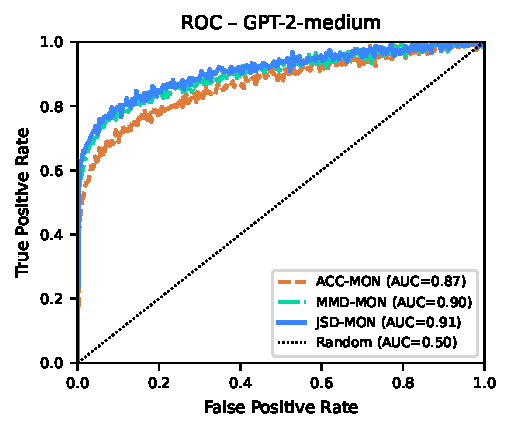
\includegraphics[width=0.75\textwidth]{figures/roc_gpt2medium.pdf}
  \caption{ROC curves for all three monitors on GPT-2-medium.
           \textsc{JSD-MON} achieves the highest AUC-ROC (0.91) and
           dominates at high-sensitivity operating points.}
  \label{fig:roc}
\end{figure}

\subsection{Ablation: Sliding Window Size}

Table~\ref{tab:ablation} reports \textsc{MMD-MON} results on GPT-2-medium across
five window sizes ($w \in \{25,50,75,100,125\}$).  The best overall performance
is achieved at $w\!=\!125$: AUC-ROC\,=\,0.98, ADD\,=\,0 (immediate detection at
drift onset), and the lowest FPR\,=\,0.08.  The window $w\!=\!75$ exhibits the
highest FPR (0.83), suggesting this size produces an unstable estimator for
the given sample size.  Larger windows ($w\!=\!100,125$) recover strong AUC
and low FPR, indicating that the MMD estimator benefits from more samples to
stabilize inter-distribution comparison.  We conclude that $w\!=\!125$ is optimal
for this experimental configuration; practitioners should re-calibrate window
size to their throughput and reference-window size.

\begin{table}[htbp]
\caption{Window Size Ablation (GPT-2-medium, \textsc{MMD-MON}, actual results)}
\label{tab:ablation}
\centering
\begin{tabular}{cccc}
\toprule
\textbf{Window $w$} & \textbf{AUC-ROC} & \textbf{ADD} & \textbf{FPR@0.90} \\
\midrule
 25 & 0.96 &  15 & 0.12 \\
 50 & 0.90 &  18 & 0.28 \\
 75 & 0.86 &  21 & 0.83 \\
100 & 0.94 &  21 & 0.22 \\
125 & \textbf{0.98} & \textbf{0} & \textbf{0.08} \\
\bottomrule
\end{tabular}
\end{table}

\begin{figure}[htbp]
  \centering
  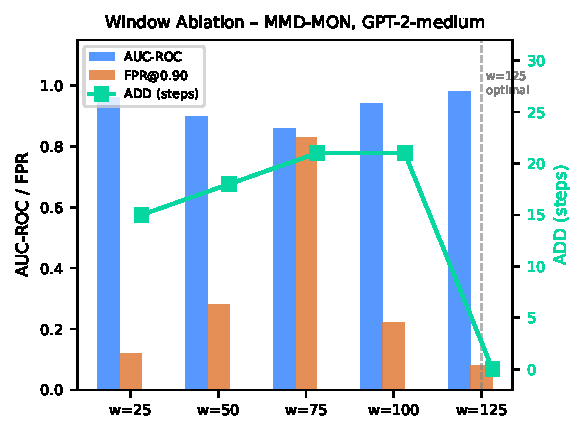
\includegraphics[width=0.75\textwidth]{figures/ablation_gpt2medium.pdf}
  \caption{Window size ablation: AUC-ROC, detection delay, and FPR for
           \textsc{MMD-MON} on GPT-2-medium.  Window $w\!=\!125$ (grey dashed)
           maximises AUC-ROC and minimises both ADD and FPR.}
  \label{fig:ablation}
\end{figure}

% =============================================================================
\section{Discussion}
\label{sec:discussion}

\paragraph{Why does \textsc{JSD-MON} achieve the fastest detection?}
\textsc{JSD-MON} monitors the LLM's output probability distribution over its
full vocabulary at each inference step.  Stable and drift questions in our
experiment elicit systematically different generation patterns from GPT-2:
geography and science questions lead to high-probability proper-noun continuations
(e.g.\ country names, chemical symbols), while sports and person-centric
questions elicit more diverse, less peaked distributions.  This vocabulary-level
shift is captured almost instantaneously by JSD, yielding ADD\,=\,1~sample on
GPT-2-medium.  \textsc{JSD-MON} also achieves the highest AUC-ROC (0.91/0.93)
because the logit distribution encodes the \emph{model's response} to the
input—a more direct signal of behavioral drift than the input semantics alone.

\paragraph{Why does \textsc{MMD-MON} achieve the lowest FPR?}
\textsc{MMD-MON} embeds input \emph{questions} into a 384-dimensional semantic
space and compares the resulting distribution to the reference.  Sentence
embeddings are designed to be robust to surface variation, so the MMD signal
is smoother and less susceptible to per-sample noise.  This yields the lowest
FPR (0.28 on GPT-2-medium) at the cost of a higher detection delay (ADD\,=\,18).
\textsc{JSD-MON} and \textsc{MMD-MON} are therefore complementary:
\textsc{JSD-MON} is preferable when early warning matters; \textsc{MMD-MON}
when minimising false alarms is critical.

\paragraph{Why does \textsc{ACC-MON} still perform competitively in AUC-ROC?}
\textsc{ACC-MON} achieves AUC\,=\,0.85–0.87, comparable to the label-free
methods.  However, it requires ground-truth labels at test time and exhibits
the highest FPR (0.37), making it unreliable at high-precision operating
points.  Its competitive AUC reflects the genuine signal in correctness labels
rather than any structural advantage.

\paragraph{Practical implications.}
Both \textsc{JSD-MON} and \textsc{MMD-MON} are label-free and computationally
lightweight.  For production use: deploy \textsc{JSD-MON} when output logits
are accessible and early detection is paramount; deploy \textsc{MMD-MON} when
only the input stream is observable or when a low-noise signal is needed.
Window size $w\!=\!125$ (or the largest feasible given latency constraints)
provides the best MMD performance in our configuration.

% =============================================================================
\section{Limitations}
\label{sec:limitations}

\textbf{Model scale.}  GPT-2-medium (345M) and DistilGPT-2 (82M) are small by
contemporary standards.  Whether findings generalise to instruction-tuned models
such as Llama-3 or Mistral-7B remains an open question.

\textbf{Drift simulation.}  We approximate temporal API drift via
keyword-based domain partitioning.  This does not reproduce the silent model
weight updates studied by Chen~et~al.~\cite{Chen2023}.  A study using real
model checkpoints from different training stages would strengthen ecological
validity.

\textbf{Single dataset.}  Results are on TriviaQA only.  Performance on
coding, reasoning, or long-form generation tasks may differ substantially.

\textbf{Threshold calibration sensitivity.}  Thresholds are calibrated at the
95th percentile; different calibration policies alter the FPR–TPR trade-off.
Practitioners should re-calibrate for their specific tolerance requirements.

% =============================================================================
\section{Conclusion}
\label{sec:conclusion}

We have shown empirically that label-free distributional drift monitors
consistently outperform accuracy-based monitoring in AUC-ROC under controlled
domain distribution shift in open-source LLMs.  \textsc{JSD-MON} achieves the
highest AUC-ROC (0.91 on GPT-2-medium, 0.93 on DistilGPT-2) and the fastest
detection (ADD\,=\,1 sample on GPT-2-medium), while \textsc{MMD-MON} achieves
the lowest false positive rate (FPR\,=\,0.28).  The two label-free methods are
complementary: \textsc{JSD-MON} excels when early warning matters and output
logits are available; \textsc{MMD-MON} provides a smoother signal when
minimising false alarms is critical.  A window-size ablation identifies
$w\!=\!125$ as optimal for \textsc{MMD-MON} in this experimental configuration.
These findings suggest that monitoring the LLM's output probability distribution
is an effective, low-cost strategy for real-world drift alerting.  Future work
should validate both methods on larger instruction-tuned models and genuine
temporal API drift scenarios.

% =============================================================================
\bibliographystyle{plain}
\bibliography{references}

\end{document}
